\documentclass[preprint,12pt,authoryear]{elsarticle}
\usepackage[utf8]{inputenc}
\usepackage[margin=2cm]{geometry}
\usepackage{graphicx}
\usepackage{multirow}
\usepackage{amssymb}
\usepackage{amsmath}
\usepackage{setspace}
\usepackage{outlines}
\usepackage{enumitem}
\usepackage{xcolor}
\usepackage{upgreek}
\usepackage{mathabx}
\usepackage{algorithm}
\usepackage{algorithmic}
\usepackage{amsthm}
\usepackage[labelfont=bf,font=small]{caption}
\usepackage{epsfig}
\usepackage{geometry}
\usepackage{subfigure}
\usepackage[textsize=tiny]{todonotes}
\usepackage[normalem]{ulem}
\usepackage{lipsum}
\usepackage{array}
\usepackage{booktabs}
\usepackage{lineno}
\usepackage{array}
\usepackage{tikz}
\usepackage[english]{babel}
\usepackage{animate}
\usepackage{cancel}

\usepackage[]{siunitx}
\sisetup{range-units=single,separate-uncertainty = true,print-unity-mantissa=false,per-mode=symbol,range-phrase = \text{--},
inter-unit-product=\cdot
}

\usepackage[
    protrusion=true,
    activate={true,nocompatibility},
    final,
    tracking=true,
    kerning=true,
    spacing=true,
    factor=1100]{microtype}
    
\SetTracking{encoding={*}, shape=sc}{40}

\usepackage{outlines}
\usepackage{enumitem}

\definecolor{lightblue}{rgb}{0.63, 0.74, 0.78}
\definecolor{seagreen}{rgb}{0.18, 0.42, 0.41}
\definecolor{orange}{rgb}{0.85, 0.55, 0.13}
\definecolor{silver}{rgb}{0.69, 0.67, 0.66}
\definecolor{rust}{rgb}{0.72, 0.26, 0.06}
\definecolor{purp}{RGB}{68, 14, 156}

\definecolor{zblue}{RGB}{8,81,156}
\definecolor{zpurp}{RGB}{84,39,143}
\definecolor{zred}{RGB}{165,15,21}

\colorlet{lightrust}{rust!50!white}
\colorlet{lightorange}{orange!25!white}
\colorlet{lightlightblue}{lightblue}
\colorlet{lightsilver}{silver!30!white}
\colorlet{darkorange}{orange!75!black}
\colorlet{darksilver}{silver!65!black}
\colorlet{darklightblue}{lightblue!65!black}
\colorlet{darkrust}{rust!85!black}
\colorlet{darkseagreen}{seagreen!85!black}



\usepackage{hyperref}
\hypersetup{
  colorlinks=true,
}
\usepackage{tabularx}
\usepackage{bbm}
\usepackage{bm}

\usepackage[nameinlink]{cleveref}
\crefname{equation}{}{}
\def\appendixname{}
\crefname{appendix}{}{}


\usepackage{setspace}
% \doublespacing
\setlength{\heavyrulewidth}{1.5pt}
% \setlength{\abovetopsep}{4pt}
 
\usepackage{soul}
\sethlcolor{yellow}

\usepackage[parfill]{parskip}

\usepackage{lineno}
\usepackage{tcolorbox}
%\linenumbers

%% Self-defined Macros
\newcommand{\bn}[1]{\mathbf{#1}}
\newcommand{\bs}[1]{\ensuremath{\boldsymbol{#1}}}
\newcommand{\mc}[1]{\ensuremath{\mathcal{#1}}}
\newcommand{\norm}[1]{\ensuremath \lVert #1 \rVert}
\newcommand{\GD}[1]{ D #1 (\boldsymbol{F})[\boldsymbol{H}]}
\newcommand{\GDI}[1]{ D #1 (\boldsymbol{I})[\boldsymbol{H}]}
\newcommand{\Lin}[1]{ L_{\boldsymbol{F}} #1 [\boldsymbol{H}]}
\newcommand{\LinI}[1]{ L_{\boldsymbol{I}} #1 [\boldsymbol{H}]}
\newcommand{\Dm}[1]{\ensuremath{\boldsymbol{\varphi} } }
\newcommand{\tr}[1]{\textcolor{red}{#1}}
\newcommand{\ignore}[1]{}
\newcommand{\fracp}[2]{\frac{\partial #1}{\partial #2}}
\newcommand{\wt}[1]{\widetilde{#1}}
\renewcommand{\[}{\left[}
\renewcommand{\]}{\right]}
\renewcommand{\(}{\left(}
\renewcommand{\)}{\right)}
\newcommand{\tn}{\textnormal}
\newcommand{\gradX}{\nabla_{\bm{X}}}
\newcommand{\gradx}{\nabla_{\bm{x}}}
\newcommand{\gradF}{\nabla_{\bn{F}}}

%\newcommant{\pfrac[2]}{\frac{\partial {#1}}{\partial {#2}}}

%% Coloring for comments
\usepackage{color,tikz,soul}
\newcommand{\jbe}[1]{\textcolor{violet}{#1}}

\newcommand{\rev}[1]{\textcolor{red}{#1}}

\usepackage{xcolor, soul}
\sethlcolor{yellow}
\usepackage[per-mode=symbol]{siunitx}

\setlength{\tabcolsep}{12pt}

\renewcommand{\thetable}{\arabic{table}} % Originally Roman uppercase

\journal{ME517---Mechanics of Soft Materials}
\setlength{\marginparwidth}{2cm}
\newcommand\C[1]\null %\C{for inline comments}
\begin{document}

% \include{instr-part1}
\section{Statement of Research Interest}
Microtubules are a core component of the cellular cytoskeleton, a network of filaments in cells that contribute to varied mechanical processes including shape maintenance, force generation, and motility. Microtubule networks are generally acknowledged as displaying viscoelastic behavior, attributed to the collective behavior of the network [\cite{visco_review, visco_MTs}]. Other cytoskeletal filaments (including actin and intermediate filaments) are also well-known as being viscoelastic. However, the individual microtubules themselves are commonly treated as elastic due to their high stiffness relative to other cytoskeletal filaments. Yet, there are some behaviors of individual microtubules (notably, for certain types and compositions of microtubules) that cannot be explained by a purely elastic model. Single microtubules show increased deformation over time with repeated bending by the same hydrodynamic force, as well as a length-dependent persistence length [\cite{acetyl_aging, Celeg_lumen}]. Therefore, I propose a project exploring the potential viscoelastic properties of individual microtubules. In this project, I would first characterize the (potential) viscoelastic properties of microtubules using active bending experiments in an optical trap. Then, I would explore the mechanisms by which the viscoelastic properties of microtubules arise---or, in the case that microtubules do not generally show viscoelastic properties, the mechanisms by which some microtubules demonstrate certain viscoelastic properties like relaxation.

I am interested in studying this topic for two main reasons. First, I am very interested in mechanobiology as a field and want to better understand the mechanical properties of biological systems. Second, I want to bring a stronger physical and mechanical perspective to my current research on microtubule mechanics. There are a lot of papers noting how the mechanical properties of microtubules are more complex than a simple homogeneous rod, so I want to push this idea a little further by actually applying it to experiments. Hopefully, doing so will allow a better understanding of how microtubules respond to and generate forces in cells, as well as how their molecular composition (for example, microtubules are made of thinner protofilaments which have lateral interactions of a different strength than the longitudinal interactions that build the protofilaments) ends up resulting in their mechanical properties.


% bring this physical and mechanical perspective to my current research with microtubules.

% I am interested in studying the viscoelastic properties of individual microtubules for a couple of reasons. First of all, I am really interested in mechanobiology and how biological systems have adapted to work around or use physical forces. I am currently in a microtubule-focused lab that is well-equipped to study how different microtubule vary in their properties (based on different compositions or biochemical modifications). The lab also does research on kinesin motors and does have the ability to do whole cell (which could add to microtubule network studies) experiments as well. I want to bring my mechanical interests and physics background into my research more strongly. Plus, the lab has an optical trap that is well-suited to single molecule (or network) studies of microtubules, which I'm hoping to use to help bring a more mechanical and soft materials perspective to my research.

% Microtubules are a core component of the cellular cytoskeleton, a network of intracellular filaments that participate in or contribute to various mechanical processes including shape maintenance, force generation, and cell motility. Microtubule networks are acknowledged as having viscoelastic behavior, generally attributed to being an emergent property from the collective behavior of the network [\cite{visco_review, visco_MTs}]. As the stiffest of the cytoskeletal filaments, microtubule deformation is commonly treated as that of a stiff, elastic rod (citation). However, some microtubules also demonstrate behaviors inconsistent with a purely elastic filament, and which indicate that individual microtubules might also exhibit viscoelastic behaviors. For example, after repeated bending through hydrodynamic flow, certain varieties of microtubules will demonstrate increased bending deformation under the same applied flow force and therefore show relaxation upon repeated force application [\cite{acetyl_aging}]. In addition, some microtubules show a length-dependence in measured persistence length, an idea inconsistent with the buckling of an isotropic elastic rod [\cite{Celeg_lumen}]. Therefore, I would like to explore the viscoelastic properties of individual microtubules, first characterizing these properties and then exploring the mechanisms by which these viscoelastic properties arise for certain microtubule varieties. This would be done by optical trapping (like bending microtubules, condense and fit this in more clearly).

\section{Intellectual Merit}
Microtubules and their mechanical properties are addressed across many experimental and computational papers. However, there is both a wide range of experimentally measured values for microtubule stiffness and a limited understanding of how microtubules establish their mechanical properties. This is an especially interesting question because recent papers have noted that microtubules of different chemical compositions display different mechanical properties [\cite{Celeg_lumen}]. Determining whether individual microtubules display viscoelastic properties has the potential to address the current discrepancies between mechanical measurements focused on finding a single elastic modulus by more wholistically describing the mechanical properties of microtubules. Even if individual microtubules are not viscoelastic (which is absolutely possible!), establishing this concretely will allow further investigation of the select viscoelastic properties microtubules \emph{do} display. Regardless of the results, a better understanding of how individual microtubules behave in response to different mechanical stimuli (such as varied loading rates, repeated loading, or deformation directions) will develop our understanding of how microtubules actually deform in conditions where they do not form cross-linked networks (for example, filamentous bundles or single microtubules). 

In this course, lecture materials on viscoelastic bending and experimental techniques used to characterize the soft material properties of actual physical systems will be beneficial to this research proposal. Discussions of how to differentiate elastic from viscoelastic behavior and concerning the viscoelastic behaviors of thin filaments will be particularly applicable.


% At least based on my current understanding of mechanics, course materials on viscoelastic bending and experimental techniques used to characterize the soft material properties of a system will be related to (and help propose) this research idea.
%in contrast, actin filaments have a consistently charachterized bending stiffness/mechanical behaviors in response to forces; mechanical properties and behaviors; in different conditions (such as different microtubule lengths) 
% Microtubules and their mechanical properties have been the subject of numerous experiments and physical models (citations). However, there is a limited understanding of where microtubule mechanics come from and how they might vary under different circumstances. In particular, current mechanical measurements and models show highly conflicting results in measured bending stiffness and other mechanical properties. A better understanding of microtubule mechanics by investigating whether they act as viscoelastic systems could serve to resolve some of these conflicts by (explaining? addressing? providing a potential explanation or expansion on the current model?) expanding the current models of microtubule bending to include more complex behaviors. That is, characterizing the viscoelastic properties of individual microtubules will provide a more robust understanding of how microtubules behave mechanically--or the lack thereof will hint to another mechanism governing the uncertainty in how they behave mechanically. A better understanding of how microtubules behave mechanically in different conditions will also help understand how microtubules actually deform in cells under conditions where they do not form networks with crosslinking that would lead to emergent viscoelasticity. For example, understanding how microtubule bundles or other filamentous formations (more filamentous microtubule bundles rather than crosslinked mesh networks with known viscoelastic behavior responses) behave mechanically. And how they experience different forces and respond under different conditions in ways that could impact cell function and mechanics in different conditions. Also understand how microtubules age and change mechanically over time as they exist in cells and are subject to repeated bending (if not dynamic??) over time in the cell.

% Relaxation of bending? Definitely go back to the syllabus a bit more. different lens as well? emergent vs induvidual property at a broader scale? better understanding of MT mechanics to resolve conflicting measurements--made under different conditions? also better understanding of how MTs actually deform in cells in different conditions and that experience different forces--like how it could tell us whether we expect there to be other VE properties that could impact cell function, mechanics, etc.

\section{Broader Impact}
In many non-dividing cell types, microtubules are relatively long-lasting and therefore subject to repeated stressing and bending. Better understanding the mechanics of microtubules would contribute to understanding the functional roles of microtubules in such cell types. For example, cardiomyocytes are specialized cells important for the repeated contractions of the heart. In these cells, there are also microtubules that are both essential to these contractions and that have to endure repeated bending and straightening [\cite{cardmy_review}]. A better understanding of how microtubules deform in response to stress could allow us to better understand the mechanics of hear muscle contraction. In addition, understanding what mechanical of microtubules properties are necessary for proper heart function has the potential to be used in health applications, as the mechanical modulation of microtubules has been proposed as a potential therapeutic target in heart failure [\cite{card_HF}]. 

% In non-dividing cells, certain microtubules are subject to repeated stressing and bending. For example, cardiomyocytes are specialized heart cells important in contraction. In these cells, microtubules are also repeatedly bent and straightened from this repeated contraction [\cite{cardmy_review}]. With the stiffness of this microtubule network important to the proper function of the heart, a better understanding of how individual microtubules bend and more specifically how their bending properties change with this repeated deformation could contribute to a better understanding of their overall function in the heart [\cite{card_HF}]. In addition, deviations from expected relaxation behavior could point to new proteins responsible for maintaining proper microtubule flexibility with repeated bending.
% (this might be a stretch) In addition, neurons have long-lived microtubules that are part of transport (more on this). While these microtubules do not serve a primary role in (resisting?) mechanics, (time-dependent) changes in the microtubule material properties over time due to forces--whether external or from (on the smaller scale of, could test both force ranges) intracellular interactions with transport molecules or the crowded cytoplasm would be important in the resistance of the microtubules to breakage? Since 

% can help differentiate effects of the microtubule itself and proteins that help to offset bending with age like acetylation or MAPS

% While studies exist that investigate the roles of MAPs and crowding in stabilizing microtubules. how contributes to society like health applications vs better understanding of some phenomena folks are interested in understanding
% oh but more stiff is part of heart failure
% Better understanding of how microtubules age over time. Bundles of microtubules
% Potential for platelets and cardiomyocytes that have constantly bent (are these dynamic?) microtubules or repeated mechanical contractions respectively.


\begin{thebibliography}{00}

% using Chicago 18th shortened from Zotero
\bibitem[Corominas-Murtra and Petridou, 2021]{visco_review}
Corominas-Murtra, Bernat, and Nicoletta I. Petridou. “Viscoelastic Networks: Forming Cells and Tissues.” Frontiers in Physics 9 (2021). https://doi.org/10.3389/fphy.2021.666916.
\bibitem[Lin et al., 2007]{visco_MTs}
Lin, Yi-Chia, Gijsje H. Koenderink, Frederick C. MacKintosh, and David A. Weitz. “Viscoelastic Properties of Microtubule Networks.” Macromolecules 40, no. 21 (2007): 7714–20. https://doi.org/10.1021/ma070862l.
\bibitem[Portran et al., 2017]{acetyl_aging}
Portran, Didier, Laura Schaedel, Zhenjie Xu, Manuel Théry, and Maxence V. Nachury. “Tubulin Acetylation Protects Long-Lived Microtubules against Mechanical Ageing.” Nature Cell Biology 19, no. 4 (2017): 391–98. https://doi.org/10.1038/ncb3481.
\bibitem[Yucheng et al., 2025]{Celeg_lumen}
Ye, Yucheng, Zheng Hao, Jingyi Luo, et al. “Tubulin Isotypes of C. Elegans Harness the Mechanosensitivity of the Lattice for Microtubule Luminal Accessibility.” Nature Physics, ahead of print (2025). https://doi.org/10.1038/s41567-025-02983-w.
\bibitem[Uchida et al., 2022]{cardmy_review}
Uchida, Keita, Emily A. Scarborough, and Benjamin L. Prosser. “Cardiomyocyte Microtubules: Control of Mechanics, Transport, and Remodeling.” Annual Review of Physiology 84, no. Volume 84, 2022 (2022): 257–83. https://doi.org/10.1146/annurev-physiol-062421-040656.
\bibitem[Caporizzo and Prosser, 2022]{card_HF}
Caporizzo, Matthew A., and Benjamin L. Prosser. “The Microtubule Cytoskeleton in Cardiac Mechanics and Heart Failure.” Nature Reviews Cardiology 19, no. 6 (2022): 364–78. https://doi.org/10.1038/s41569-022-00692-y.
\bibitem[Okenve-Ramos et al, 2024]{neur_aging}
Okenve-Ramos, Pilar, Rory Gosling, Monika Chojnowska-Monga, et al. “Neuronal Ageing Is Promoted by the Decay of the Microtubule Cytoskeleton.” PLOS Biology 22, no. 3 (2024): e3002504. https://doi.org/10.1371/journal.pbio.3002504.

\bibliographystyle{elsarticle-harv} 
% \bibliography{cas-refs}
\end{thebibliography}

% \documentclass[preprint,12pt,authoryear]{elsarticle}
% \usepackage[utf8]{inputenc}
\usepackage[margin=2cm]{geometry}
\usepackage{graphicx}
\usepackage{multirow}
\usepackage{amssymb}
\usepackage{amsmath}
\usepackage{setspace}
\usepackage{outlines}
\usepackage{enumitem}
\usepackage{xcolor}
\usepackage{upgreek}
\usepackage{mathabx}
\usepackage{algorithm}
\usepackage{algorithmic}
\usepackage{amsthm}
\usepackage[labelfont=bf,font=small]{caption}
\usepackage{epsfig}
\usepackage{geometry}
\usepackage{subfigure}
\usepackage[textsize=tiny]{todonotes}
\usepackage[normalem]{ulem}
\usepackage{lipsum}
\usepackage{array}
\usepackage{booktabs}
\usepackage{lineno}
\usepackage{array}
\usepackage{tikz}
\usepackage[english]{babel}
\usepackage{animate}
\usepackage{cancel}

\usepackage[]{siunitx}
\sisetup{range-units=single,separate-uncertainty = true,print-unity-mantissa=false,per-mode=symbol,range-phrase = \text{--},
inter-unit-product=\cdot
}

\usepackage[
    protrusion=true,
    activate={true,nocompatibility},
    final,
    tracking=true,
    kerning=true,
    spacing=true,
    factor=1100]{microtype}
    
\SetTracking{encoding={*}, shape=sc}{40}

\usepackage{outlines}
\usepackage{enumitem}

\definecolor{lightblue}{rgb}{0.63, 0.74, 0.78}
\definecolor{seagreen}{rgb}{0.18, 0.42, 0.41}
\definecolor{orange}{rgb}{0.85, 0.55, 0.13}
\definecolor{silver}{rgb}{0.69, 0.67, 0.66}
\definecolor{rust}{rgb}{0.72, 0.26, 0.06}
\definecolor{purp}{RGB}{68, 14, 156}

\definecolor{zblue}{RGB}{8,81,156}
\definecolor{zpurp}{RGB}{84,39,143}
\definecolor{zred}{RGB}{165,15,21}

\colorlet{lightrust}{rust!50!white}
\colorlet{lightorange}{orange!25!white}
\colorlet{lightlightblue}{lightblue}
\colorlet{lightsilver}{silver!30!white}
\colorlet{darkorange}{orange!75!black}
\colorlet{darksilver}{silver!65!black}
\colorlet{darklightblue}{lightblue!65!black}
\colorlet{darkrust}{rust!85!black}
\colorlet{darkseagreen}{seagreen!85!black}



\usepackage{hyperref}
\hypersetup{
  colorlinks=true,
}
\usepackage{tabularx}
\usepackage{bbm}
\usepackage{bm}

\usepackage[nameinlink]{cleveref}
\crefname{equation}{}{}
\def\appendixname{}
\crefname{appendix}{}{}


\usepackage{setspace}
% \doublespacing
\setlength{\heavyrulewidth}{1.5pt}
% \setlength{\abovetopsep}{4pt}
 
\usepackage{soul}
\sethlcolor{yellow}

\usepackage[parfill]{parskip}

\usepackage{lineno}
\usepackage{tcolorbox}
%\linenumbers

% %% Self-defined Macros
\newcommand{\bn}[1]{\mathbf{#1}}
\newcommand{\bs}[1]{\ensuremath{\boldsymbol{#1}}}
\newcommand{\mc}[1]{\ensuremath{\mathcal{#1}}}
\newcommand{\norm}[1]{\ensuremath \lVert #1 \rVert}
\newcommand{\GD}[1]{ D #1 (\boldsymbol{F})[\boldsymbol{H}]}
\newcommand{\GDI}[1]{ D #1 (\boldsymbol{I})[\boldsymbol{H}]}
\newcommand{\Lin}[1]{ L_{\boldsymbol{F}} #1 [\boldsymbol{H}]}
\newcommand{\LinI}[1]{ L_{\boldsymbol{I}} #1 [\boldsymbol{H}]}
\newcommand{\Dm}[1]{\ensuremath{\boldsymbol{\varphi} } }
\newcommand{\tr}[1]{\textcolor{red}{#1}}
\newcommand{\ignore}[1]{}
\newcommand{\fracp}[2]{\frac{\partial #1}{\partial #2}}
\newcommand{\wt}[1]{\widetilde{#1}}
\renewcommand{\[}{\left[}
\renewcommand{\]}{\right]}
\renewcommand{\(}{\left(}
\renewcommand{\)}{\right)}
\newcommand{\tn}{\textnormal}
\newcommand{\gradX}{\nabla_{\bm{X}}}
\newcommand{\gradx}{\nabla_{\bm{x}}}
\newcommand{\gradF}{\nabla_{\bn{F}}}

%\newcommant{\pfrac[2]}{\frac{\partial {#1}}{\partial {#2}}}

%% Coloring for comments
\usepackage{color,tikz,soul}
\newcommand{\jbe}[1]{\textcolor{violet}{#1}}

\newcommand{\rev}[1]{\textcolor{red}{#1}}

\usepackage{xcolor, soul}
\sethlcolor{yellow}
\usepackage[per-mode=symbol]{siunitx}

\setlength{\tabcolsep}{12pt}

\renewcommand{\thetable}{\arabic{table}} % Originally Roman uppercase

% \journal{ME517---Mechanics of Soft Materials}
% \setlength{\marginparwidth}{2cm}
% \begin{document}

\section*{Examples I. Mathematical Preliminaries}
\label{PS1}

\bigskip
\subsection*{1--1. \textbf{Convolutional integrals} [4 pts].}

Writing out the Laplace transform of $\varepsilon(t)$ without any specific $\sigma(t)$ function gives the expression
\begin{equation}
    \mathcal{L}\{\varepsilon(t)\} = \mathcal{L}\{ \int_0^t J(t-\tau) \frac{d\sigma(\tau)}{d\tau} d\tau \}.
\end{equation}

The general function provided for $\varepsilon(t)$ is a convolution in the form 
\begin{equation}
    (f \ast g)(t) = \int_0^t{f(\tau)g(t-\tau)d\tau}
\end{equation}
with signal function $f(\tau) = \frac{d\sigma(\tau)}{d\tau}$ and filter function $g(t-\tau) = J(t-\tau)$. The Laplace transform of a convolution is the product of the individual Laplace transforms for the two convolved functions:
\begin{equation}
    \mathcal{L}\{\varepsilon(t)\} = \mathcal{L}\{ (J \ast f)(t)\} = J(s)F(s) = \mathcal{L}\{J(t)\} \space \mathcal{L}\{\frac{d\sigma(t)}{d\tau}\}.
\end{equation}
We can then evaluate the Laplace transforms for $J(t)$ and $\frac{d\sigma(t)}{d\tau}$ separately. For $J(t)$:
\begin{equation}
    \mathcal{L}\{J(t)\} = \mathcal{L}\{ J_\infty + (J_0-J_\infty)\exp[-t/\tau_c] \} = \mathcal{L}\{ J_\infty + J_0\exp[-t/\tau_c] - J_\infty\exp[-t/\tau_c]\}
\end{equation}
We use the property of linearity for the Laplace transform $\mathcal{L}\{ af(t) + bg(t)\} = a\mathcal{L}\{f(t)\} + b\mathcal{L}\{g(t)\}$, evaluate the resulting individual Laplace transforms using the table of common Laplace transforms in the notes, and then simplify to get:

\begin{equation}
\begin{split}
        \mathcal{L}\{J(t)\} = \mathcal{L}\{ J_\infty\} + \mathcal{L}\{J_0\exp[-t/\tau_c]\} + \mathcal{L}\{-J_\infty\exp[-t/\tau_c]\} \\
        = J_\infty\mathcal{L}\{ 1\} + J_0\mathcal{L}\{\exp[-t/\tau_c]\} -J_\infty\mathcal{L}\{\exp[-t/\tau_c]\} \\
        =J_\infty (1/s) + J_0 \frac{1}{s+1/\tau_c} - J_\infty \frac{1}{s+1/\tau_c} \\
        =\frac{J_\infty}{s} + (J_0-J_\infty)(\frac{1}{s+1/\tau_c}) \\
        =\frac{J_\infty}{s} + (J_0-J_\infty)(\frac{\tau_c}{s\tau_c+1})
\end{split}
\end{equation}
For the Laplace transform of $\frac{d\sigma(t)}{d\tau}$, this will depend on what loading function $\sigma(t)$ we use.

\medskip
(a) step load $\sigma_1(t) = \sigma_0 H(t)$ \newline
Using the derivative property for the Laplace transform $\mathcal{L}\{\frac{d}{dt}f(t)\} = sF(s)-f(0)$ and then simplifying we get:
\begin{equation}
\begin{split}
    \mathcal{L}\{\frac{d\sigma_1(t)}{dt}\} = s\mathcal{L}\{ \sigma_1(t)\}-\sigma_1(0) \\
    = s\mathcal{L}\{ \sigma_0H(t)\}-\sigma_0H(0) \\ 
    = s\sigma_0\mathcal{L}\{ H(t)\}-\sigma_0
\end{split}
\end{equation}
Then using that $H(0) = 1$ (note the value of 1 rather than 1/2) and $\mathcal{L}\{ H(t)\}=1/s$ we get:
\begin{equation}
\begin{split}
    \mathcal{L}\{\frac{d\sigma_1(t)}{dt}\} = s\sigma_0(1/s)-\sigma_0 = \sigma_0 - \sigma_0 = 0
\end{split}
\end{equation}
Putting this value of $\mathcal{L}\{\frac{d\sigma(t)}{dt}\}$ and the previous value of $\mathcal{L}\{J(t)\}$ (which is the same for any $\sigma(t)$) into the format of $\mathcal{L}\{\varepsilon(t)\}$ from equation (3) we get:

\begin{equation}
    \mathcal{L}\{\varepsilon_1(t)\} = \mathcal{L}\{J(t)\} \mathcal{L}\{\frac{d\sigma_1(t)}{dt}\} = 0
\end{equation}
\hspace*{\fill} $\mathcal{L}\{\varepsilon_1(t)\} = 0$ $\space \bigstar$

\medskip
(b) a sinusoidal load $\sigma_2(t) = \sigma_0  \sin(\omega t)$ \newline
Once again, we start from the general form from equation (3):
\begin{equation}
        \mathcal{L}\{\varepsilon_2(t)\} = \mathcal{L}\{J(t)\} \mathcal{L}\{\frac{d\sigma_2(t)}{dt}\}
\end{equation}
Repeating the same general ideas as for part (a) but using that $\mathcal{L}\{ \sin(at)\} = \frac{a}{s^2 + a^2}$ we get:
\begin{equation}
\begin{split}
    \mathcal{L}\{\frac{d\sigma_2(t)}{dt}\} = s\mathcal{L}\{ \sigma_2(t)\}-\sigma_2(0) \\
    = s\mathcal{L}\{ \sigma_0\sin(\omega t)\}-\sigma_0\sin(0) \\ 
    = s\sigma_0\mathcal{L}\{ \sin(\omega t)\} \\
    = s \sigma_0 (\frac{\omega}{s^2 + \omega^2}) = \frac{s \sigma_0 \omega}{s^2 + \omega^2}
\end{split}
\end{equation}
Then putting this into our equation for $\mathcal{L}\{\varepsilon_2(t)\}$:
\begin{equation}
    \mathcal{L}\{\varepsilon_2(t)\} = [\frac{J_\infty}{s} + (J_0-J_\infty)(\frac{\tau_c}{s\tau_c+1})][\frac{s \sigma_0 \omega}{s^2 + \omega^2}] \\
    =[J_\infty + (J_0-J_\infty)(\frac{s \tau_c}{s\tau_c+1})][\frac{\sigma_0 \omega}{s^2 + \omega^2}]
\end{equation}
\hspace*{\fill} $\mathcal{L}\{\varepsilon_2(t)\} = [J_\infty + (J_0-J_\infty)(\frac{s \tau_c}{s\tau_c+1})][\frac{\sigma_0 \omega}{s^2 + \omega^2}]$ $\space \bigstar$


\newpage
\bigskip
\subsection*{1--2. \textbf{Index notation} [4 pts].} Let $\bm{p}, \bm{q}, \bm{r}, \bm{a}, \bm{b}$ be vector fields on $\mathbbm{R}^3$ and $\bn{Q}$ be a change-of-basis tensor on $\mathbbm{R}^3$. Show the following identities to be true using index notation. 

\medskip
(a) $\bm{p} \times (\bm{q} \times \bm{r}) = (\bm{r} \cdot \bm{p}) \bm{q} - (\bm{q} \cdot \bm{p}) \bm{r}$ \newline
Putting the LHS into index notation (noting that $(\bm{q} \times \bm{r})_i = \epsilon_{ijk}q_jr_k$):
\begin{equation}
    \bm{p} \times (\bm{q} \times \bm{r}) = \epsilon_{lmn}p_m(\bm{q} \times\bm{r})_n \bm{e}_l = \epsilon_{lmn}p_m(\epsilon_{njk}q_jr_k) \bm{e}_l
\end{equation}
Using that the front index of $\epsilon$ doesn't matter as long as the order is preserved (ie. $\epsilon_{lmn} = \epsilon_{nlm}$) and the identity $\epsilon_{ijk}\epsilon_{ipq} = \delta_{jp}\delta_{kq} - \delta_{jq}\delta_{kp}$ the LHS simplifies to:
\begin{equation}
    \begin{split}
    \bm{p} \times (\bm{q} \times \bm{r}) = \epsilon_{lmn}\epsilon_{njk}p_mq_jr_k \bm{e}_l = \epsilon_{nlm}\epsilon_{njk}p_mq_jr_k \bm{e}_l \\
    = (\delta_{lj}\delta_{mk} - \delta_{lk}\delta_{mj})p_mq_jr_k \bm{e}_l = \delta_{lj}\delta_{mk}p_mq_jr_k \bm{e}_l - \delta_{lk}\delta_{mj}p_mq_jr_k \bm{e}_l
    \end{split}
\end{equation}
Subbing the index l to j and m to k for the first term and l to k and m to j for the second term using the Kronecker deltas (and then swapping the free index in both terms to p, since that can be anything):
\begin{equation}
    \begin{split}
    \bm{p} \times (\bm{q} \times \bm{r}) = p_kq_jr_k \bm{e}_j - p_jq_jr_k \bm{e}_k = p_kq_pr_k \bm{e}_p - p_jq_jr_p \bm{e}_p
    \end{split}
\end{equation}
Where we can rearrange terms and then note the dot products implied by this expression and go back to direct notation to get:
\begin{equation}
    \begin{split}
    \bm{p} \times (\bm{q} \times \bm{r}) = r_kp_k q_p\bm{e}_p - q_jp_j r_p\bm{e}_p = (\bm{r} \cdot \bm{p})\bm{q} - (\bm{q} \cdot \bm{p})\bm{r}
    \end{split}
\end{equation} \qed

% Putting the RHS into index notation:
% \begin{equation}
%     \begin{split}
%     (\bm{r} \cdot \bm{p}) = r_ip_i \\
%     (\bm{r} \cdot \bm{p}) \bm{q} = r_ip_iq_j \bm{e}_j \\
%     (\bm{q} \cdot \bm{p}) \bm{r} = q_ip_ir_j \bm{e}_j \\
%     (\bm{r} \cdot \bm{p}) \bm{q} - (\bm{q} \cdot \bm{p}) \bm{r} = (r_ip_iq_j - q_ip_ir_j) \bm{e}_j
%     \end{split}
% \end{equation}

\medskip
(b) $(\bm{p} \times \bm{q}) \cdot (\bm{a} \times \bm{b}) = (\bm{p} \cdot \bm{a}) (\bm{q} \cdot \bm{b}) - (\bm{q} \cdot \bm{a})(\bm{p} \cdot \bm{b})$ \newline
Putting the LHS into index notation (using $(\bm{p} \times \bm{q}) = \epsilon_{ijk}p_jq_k\bm{e}_i$ with components $(\bm{p} \times \bm{q})_i = \epsilon_{ijk}p_jq_k$ and $(\bm{a} \times \bm{b}) = \epsilon_{lmn}a_mb_n\bm{e}_l$ with components $(\bm{a} \times \bm{b})_l = \epsilon_{lmn}a_mb_n$) we get:
\begin{equation}
\begin{split}
    (\bm{p} \times \bm{q}) \cdot (\bm{a} \times \bm{b}) = (\bm{p} \times \bm{q})_a(\bm{a} \times \bm{b})_b \delta_{ab} =  (\epsilon_{ajk}p_jq_k)(\epsilon_{bmn}a_mb_n)\delta_{ab} \\
    = (\epsilon_{ajk}p_jq_k)(\epsilon_{amn}a_mb_n) = \epsilon_{ajk}\epsilon_{amn}p_jq_ka_mb_n
\end{split}
\end{equation}
Where we can use the identity $\epsilon_{ijk}\epsilon_{ipq} = \delta_{jp}\delta_{kq} - \delta_{jq}\delta_{kp}$:
\begin{equation}
    (\bm{p} \times \bm{q}) \cdot (\bm{a} \times \bm{b}) =(\delta_{jm}\delta_{kn} - \delta_{jn}\delta_{km})p_jq_ka_mb_n = \delta_{jm}\delta_{kn}p_jq_ka_mb_n - \delta_{jn}\delta_{km}p_jq_ka_mb_n 
\end{equation}
Simplifying using the Kronecker deltas and rearranging the terms:
\begin{equation}
    (\bm{p} \times \bm{q}) \cdot (\bm{a} \times \bm{b}) = p_jq_ka_jb_k - p_jq_ka_kb_j = p_ja_jq_kb_k - q_kba_kp_jb_j
\end{equation}
Which we can put back into direct notation to get the following:
\begin{equation}
    (\bm{p} \times \bm{q}) \cdot (\bm{a} \times \bm{b}) = p_ja_jq_kb_k - q_kba_kp_jb_j = (\bm{p} \cdot \bm{a}) (\bm{q} \cdot \bm{b}) - (\bm{q} \cdot \bm{a})(\bm{p} \cdot \bm{b})
\end{equation} \qed

\medskip
(c) $(\bm{a} \otimes \bm{b})(\bm{p} \otimes \bm{q}) = \bm{a}\otimes\bm{q}(\bm{b} \cdot \bm{p}) $ \newline
Noting that the individual pieces of this expression can be written in index notation as $(\bm{a} \otimes \bm{b}) = (a_i\bm{e}_i) \otimes (b_j\bm{e}_j) = a_ib_j(\bm{e}_i \otimes\bm{e}_j)$ with components $(\bm{a} \otimes \bm{b})_{ij} = a_ib_j$ and $(\bm{p} \otimes \bm{q}) = p_kq_l(\bm{e}_k \otimes\bm{e}_l)$ with components $(\bm{p} \otimes \bm{q})_{kl} = p_kq_l$, we can write the LHS of this expression:
\begin{equation}
    (\bm{a} \otimes \bm{b})(\bm{p} \otimes \bm{q}) = a_ib_j(\bm{e}_i \otimes\bm{e}_j)p_kq_l(\bm{e}_k \otimes\bm{e}_l) = a_ib_jp_kq_l(\bm{e}_i \otimes\bm{e}_j)(\bm{e}_k \otimes\bm{e}_l)
\end{equation}
Where the two outer products at the end are multiplied as tensors ($\bn{A}=\bn{B}\bn{C}$ as $\bn{A}_{ij} = \bn{B}_{ik}\bn{C}_{kj}$) to get $\delta_{jk}(\bm{e}_i \otimes\bm{e}_l)$ and a resulting LHS expression of:
\begin{equation}
    (\bm{a} \otimes \bm{b})(\bm{p} \otimes \bm{q}) = a_ib_jp_kq_l\delta_{jk}(\bm{e}_i \otimes\bm{e}_l) = a_ib_jp_jq_l(\bm{e}_i \otimes\bm{e}_l)
\end{equation}
Where we can then rearrange our terms and bring this expression back to direct notation to get:
\begin{equation}
    (\bm{a} \otimes \bm{b})(\bm{p} \otimes \bm{q}) = a_iq_l(\bm{e}_i \otimes\bm{e}_l)b_jp_j = (\bm{a} \otimes \bm{q})(\bm{b} \cdot\bm{p}) = \bm{a} \otimes \bm{q}(\bm{b} \cdot\bm{p})
\end{equation} \qed

% Alternatively, we can also write the RHS in index notation as well and see that it is equal to 
% \begin{equation}
%     \bm{a}\otimes\bm{q}(\bm{b} \cdot \bm{p}) = (a_i\bm{e}_i) \otimes(q_j\bm{e}_jb_kp_k) = a_iq_jb_kp_k(\bm{e}_i \otimes \bm{e}_j)
% \end{equation}

% Alternatively, we can approach this question index-by-index. Noting that what we are doing on the LHS of this expression is multiplying two tensors, we can apply the rule for tensor multiplication in index notation ($\bn{A}=\bn{B}\bn{C}$ as $\bn{A}_{ij} = \bn{B}_{ik}\bn{C}_{kj}$) so that:
% \begin{equation}
%      [(\bm{a} \otimes \bm{b})(\bm{p} \otimes \bm{q})]_{ij} = (\bm{a} \otimes \bm{b})_{ik} (\bm{p} \otimes \bm{q})_{kj} = a_ib_kp_kq_j = b_kp_ka_iq_j
% \end{equation}
% If we note that $b_kp_k$ is a dot product and that $a_iq_j$ is the $ij$ component of an outer product we get:
% \begin{equation}
%     [(\bm{a} \otimes \bm{b})(\bm{p} \otimes \bm{q})]_{ij} = (\bm{a} \otimes \bm{q})_{ij}
% \end{equation}

\medskip
(d) $\bn{Q}^\intercal\bm{a} \cdot \bn{Q}^\intercal\bm{b} = \bm{a}\cdot\bm{b} $ \newline
For simplicity, let $\bn{Q}^\intercal = \bn{R}$ where $\bn{R}^\intercal = \bn{Q}$ so that the expression we are trying to prove is $\bn{R}\bm{a} \cdot \bn{R}\bm{b} = \bm{a}\cdot\bm{b}$. That is, since $\bn{Q}$ is a transformation from one basis to another (say, we can define the transformation of $\bn{Q}$ as from the $\{f_i\}$ basis to the $\{e_i\}$ basis), and $\bn{Q}^\intercal$ the reverse or inverse transformation (say $\{e_i\}$ to $\{f_i\}$), we are just defining $\bn{R}$ so that it does this inverse transformation (in our case, from $\{e_i\}$ to $\{f_i\}$). \newline
% Using that $\bn{R}_{ij} = \bm{f}^{(i)} \cdot \bm{e}^{(j)}= f^{(i)}_ke^{(j)}_k$ for $\bm{R}$ defining a transformation from $\{e_i\}$ to $\{f_i\}$ and that $\bm{R}$
Using that the transformation of a vector from $\{e_i\}$ to $\{f_i\}$ can be written in index notation as $\bm{v}^f_i = \bn{Q}_{ij}\bm{v}^e_j$, we can write the two transformed terms in the dot product as:
\begin{equation}
    \begin{split}
    [\bn{R}\bm{a}]_i = R_{ij}a^e_j = a^f_i \\
    [\bn{R}\bm{b}]_i = R_{ij}b^e_j = b^f_i
    \end{split}
\end{equation}
So then writing out the LHS:
\begin{equation}
    \bn{R}\bm{a} \cdot \bn{R}\bm{b} =[\bn{R}\bm{a}]_i[\bn{R}\bm{b}]_i = a^f_ib^f_i = \bm{a}\cdot\bm{b}
\end{equation} \qed
\newpage

\subsection*{1--3. \textbf{Tensors and vectors} [4 pts].}
Expand out the LHS by writing $\bm{u}$ as the sum of its projected components:
\begin{equation}
    \bm{u} = \bm{u}_{||} + \bm{u}_{\perp} = \bn{P}_{\bm{n}}^{||}\bm{u} + \bn{P}_{\bm{n}}^{\perp}\bm{u}
\end{equation}
Writing the parallel component $\bm{u}_{||}$ or $\bn{P}_{\bm{n}}^{||}\bm{u}$ by its definition:
\begin{equation}
    \bm{u}_{||} = (\bm{u} \cdot \bm{n}) \bm{n}
\end{equation}
And then writing the perpendicular component $\bm{u}_{\perp}$ or $\bn{P}_{\bm{n}}^{\perp}\bm{u}$ by its definition:
\begin{equation}
    \bm{u}_{\perp} = \bm{u} - \bm{u}_{||} = \bm{u} - (\bm{u} \cdot \bm{n}) \bm{n}
\end{equation}
We can then multiply $\bm{u}$ by 1 in the form $(\bm{n} \cdot \bm{n})$ and apply the identity $\bm{p} \times (\bm{q} \times \bm{r}) = (\bm{r} \cdot \bm{p})\bm{q} - (\bm{q} \cdot \bm{p})\bm{r}$:
\begin{equation}
    \bm{u}_{\perp} = (\bm{n}\cdot\bm{n})\bm{u} - (\bm{u} \cdot \bm{n}) \bm{n} = \bm{n} \times(\bm{u} \times \bm{n})
\end{equation}
Combining this expression for $\bm{u}_{\perp}$ with the prior for $\bm{u}_{||}$ gives:
\begin{equation}
    \bm{u} = \bm{u}_{||} + \bm{u}_{\perp} = (\bm{u} \cdot \bm{n}) \bm{n} + \bm{n} \times(\bm{u} \times \bm{n})
\end{equation} \qed

% Alternatively, using the tensor forms of the definition for the projection tensor (rather than the vector aspects of its definition), we can rewrite $\bm{u}_{\perp}$ as:
% \begin{equation}
%     \bm{u}_{\perp} = (\bn{I} - \bm{n} \otimes \bm{n}) \bm{u}
% \end{equation}
% Then, using the definition of an outer product $(\bm{u} \otimes\bm{v})\bm{w} = \bm{u}(\bm{v} \cdot \bm{w}) = (\bm{v} \cdot \bm{w})\bm{u}$ we get:
% \begin{equation}
%     \bm{u}_{\perp} = \bn{I}\bm{u} - (\bm{n} \cdot \bm{u})\bm{n} = 
% \end{equation}

% Writing $\bm{u}_{||}$ or $\bn{P}_{\bm{n}}^{||}\bm{u}$ by its definition $(\bm{u} \cdot \bm{n}) \bm{n}$ and $\bm{u}_{\perp}$ or $\bn{P}_{\bm{n}}^{\perp}\bm{u}$ by its definition $(\bn{I} - \bm{n} \otimes \bm{n}) \bm{u}$ we get:
% \begin{equation}
%     \bm{u} = (\bm{u} \cdot \bm{n}) \bm{n} + (\bn{I} - \bm{n} \otimes \bm{n}) \bm{u}
% \end{equation}
% Where we can rearrange the 

\newpage
\subsection*{1--4. \textbf{Vector and tensor calculus} [4 pts].}

\medskip
(a) $\gradX \times (\phi \bm{a}) = \phi \gradX \times \bm{a} + (\gradX\phi) \times \bm{a}$ \newline
Writing the cross product in the LHS in index notation we get:
\begin{equation}
    \gradX \times (\phi \bm{a}) = \epsilon_{ijk} \frac{\delta}{\delta x_j}(\phi \bm{a})_k\bm{e}_i
\end{equation}
Then applying the product rule for differentiation:
\begin{equation}
   \gradX \times (\phi \bm{a}) = \epsilon_{ijk}\bm{e}_i (\phi \frac{\partial a_k}{\partial x_j} + a_k \frac{\partial \phi}{\partial x_j}) = \epsilon_{ijk}\bm{e}_i (\phi a_{k,j} + \phi_{,j}a_k) = \epsilon_{ijk}\phi a_{k,j}\bm{e}_i + \epsilon_{ijk}\phi_{,j}a_k\bm{e}_i
\end{equation}
Where we can note that we have two cross products:
\begin{equation}
   \gradX \times (\phi \bm{a}) = \phi(\gradX \times \bm{a}) + (\phi_{,j}\bm{e}_j \times a_k\bm{e}_k)
\end{equation}
Where we also have the gradient of $\phi$ as the first term in the second cross product (that is, $\frac{\delta \phi}{\delta x_j}\bm{e}_j = \gradX \phi$) allowing us to write:
\begin{equation}
   \gradX \times (\phi \bm{a}) = \phi(\gradX \times \bm{a}) + (\gradX \phi \times \bm{a})
\end{equation} \qed

\medskip
(b)$\gradX (\bm{a} \cdot \bm{b}) = (\bm{a} \cdot \gradX) \bm{b} + (\bm{b} \cdot \gradX) \bm{a} + \bm{a} \times (\gradX \times \bm{b}) + \bm{b} \times (\gradX \times \bm{a})$ \newline
Writing the LHS in index notation and applying the product rule for differentiation:
\begin{equation}
    \gradX (\bm{a} \cdot \bm{b}) = \frac{\partial}{\partial x_i}(a_kb_k) \otimes \bm{e}_i = a_k \frac{\partial b_k}{\partial x_i} \otimes \bm{e}_i + b_k \frac{\partial a_k}{\partial x_i} \otimes \bm{e}_i = a_k b_{k,i} \bm{e}_i + b_k a_{k,i} \bm{e}_i
\end{equation}
Writing the RHS in index notation:
\begin{equation}
    \begin{split}
    (\bm{a} \cdot \gradX) \bm{b} + (\bm{b} \cdot \gradX) \bm{a} + \bm{a} \times (\gradX \times \bm{b}) + \bm{b} \times (\gradX \times \bm{a}) \\
    = (a_i\bm{e}_i \cdot \frac{\partial}{\partial x_j} \otimes \bm{e}_j)b_k\bm{e}_k + (b_i\bm{e}_i \cdot \frac{\partial}{\partial x_j} \otimes \bm{e}_j)a_k\bm{e}_k + \epsilon_{ijk}a_j(\gradX \times \bm{b})_k\bm{e}_i + \epsilon_{ijk}b_j(\gradX \times \bm{a})_k\bm{e}_i
    \end{split}
\end{equation}
Then evaluating the dot product of the basis vectors in the first and second terms and the cross products in the third and fourth terms:
\begin{equation}
    = a_i \frac{\partial}{\partial x_j}\delta_{ij}b_k\bm{e}_k + b_i\frac{\partial}{\partial x_j}\delta_{ij}a_k\bm{e}_k + \epsilon_{pqr}a_q(\epsilon_{rjk}\frac{\partial}{\partial x_j}b_k)\bm{e}_p + \epsilon_{pqr}b_q(\epsilon_{rjk}\frac{\partial}{\partial x_j}a_k)\bm{e}_p
\end{equation}
Applying the Kronecker delta and rearranging terms we get:
\begin{equation}
    = a_i b_{k,i}\bm{e}_k + b_ia_{k,i}\bm{e}_k + \epsilon_{pqr}\epsilon_{rjk}a_qb_{k,j}\bm{e}_p + \epsilon_{pqr}\epsilon_{rjk}b_qa_{k,j}\bm{e}_p
\end{equation}
Then doing a shift of the front index for each $\epsilon$, which we are allowed to do as long as the order of indicies remains the same:
\begin{equation}
    = a_i b_{k,i}\bm{e}_k + b_ia_{k,i}\bm{e}_k + \epsilon_{rpq}\epsilon_{rjk}a_qb_{k,j}\bm{e}_p + \epsilon_{rpq}\epsilon_{rjk}b_qa_{k,j}\bm{e}_p
\end{equation}
Then we can use the identity $\epsilon_{ijk}\epsilon_{ipq} = \delta_{jp}\delta_{kq} - \delta_{jq}\delta_{kp}$ to get:
\begin{equation}
    = a_i b_{k,i}\bm{e}_k + b_ia_{k,i}\bm{e}_k + (\delta_{jp}\delta_{kq} - \delta_{jq}\delta_{kp})a_qb_{k,j}\bm{e}_p + (\delta_{jp}\delta_{kq} - \delta_{jq}\delta_{kp})b_qa_{k,j}\bm{e}_p
\end{equation}
Expand:
\begin{equation}
    = a_i b_{k,i}\bm{e}_k + b_ia_{k,i}\bm{e}_k + \delta_{jp}\delta_{kq}a_qb_{k,j}\bm{e}_p - \delta_{jq}\delta_{kp}a_qb_{k,j}\bm{e}_p + \delta_{jp}\delta_{kq}b_qa_{k,j}\bm{e}_p - \delta_{jq}\delta_{kp}b_qa_{k,j}\bm{e}_p
\end{equation}
Apply the Kronecker delta:
\begin{equation}
    = a_i b_{k,i}\bm{e}_k + b_ia_{k,i}\bm{e}_k + a_kb_{k,j}\bm{e}_j - a_jb_{k,j}\bm{e}_k + b_ka_{k,j}\bm{e}_j - b_ja_{k,j}\bm{e}_k
\end{equation}
Where we can cancel the first and fourth term as well as the second and sixth term to get:
\begin{equation}
(\bm{a} \cdot \gradX) \bm{b} + (\bm{b} \cdot \gradX) \bm{a} + \bm{a} \times (\gradX \times \bm{b}) + \bm{b} \times (\gradX \times \bm{a}) = a_kb_{k,j}\bm{e}_j + b_ka_{k,j}\bm{e}_j
\end{equation}
Where if we switch all of our $j$ indices to $i$ we get:
\begin{equation}
(\bm{a} \cdot \gradX) \bm{b} + (\bm{b} \cdot \gradX) \bm{a} + \bm{a} \times (\gradX \times \bm{b}) + \bm{b} \times (\gradX \times \bm{a}) = a_kb_{k,i}\bm{e}_i + b_ka_{k,i}\bm{e}_i
\end{equation}
Which is equal to our expression for the LHS above, thereby showing that the two sides are equal. \qed

\medskip
(c) $(\bn{A} \bn{B}) \bn{:} \bn{C} = (\bn{A}^\intercal \bn{C})\bn{:} \bn{B} = (\bn{C} \bn{B}^\intercal)\bn{:} \bn{A}$ \newline
Writing the dot product on the LHS in index notation:
\begin{equation}
    (\bn{A} \bn{B}) \bn{:} \bn{C} = (A_{ij}(\bm{e}_i \otimes \bm{e}_j) \cdot B_{kl}(\bm{e}_k \otimes \bm{e}_l)) \bn{:} \bn{C} = (A_{ij}B_{kl}\delta_{jk}(\bm{e}_i \otimes \bm{e}_l)) \bn{:} \bn{C} = (A_{ij}B_{jl}(\bm{e}_i \otimes \bm{e}_l)) \bn{:} \bn{C}
\end{equation}
Then writing the contraction in index notation:
\begin{equation}
     =  (A_{ij}B_{jl}(\bm{e}_i \otimes \bm{e}_l)) \bn{:} C_{pq}(\bm{e}_p \otimes \bm{e}_q) = A_{ij}B_{jl}C_{pq}(\bm{e}_i \cdot \bm{e}_p)(\bm{e}_l \cdot \bm{e}_q) = A_{ij}B_{jl}C_{pq}\delta_{ip}\delta_{lq} = A_{ij}B_{jl}C_{il}
\end{equation}
Then we can take $\bn{A}^T$ to get:
\begin{equation}
     (\bn{A} \bn{B}) \bn{:} \bn{C} = A^T_{ji}B_{jl}C_{il} = A^T_{ji}C_{il}B_{jl}
\end{equation}
Where we can then rewrite this expression in direct notation by noting the dot product and contraction:
\begin{equation}
     (\bn{A} \bn{B}) \bn{:} \bn{C} = (\bn{A}^T\bn{C})_{jl}B_{jl} = (\bn{A}^T\bn{C})\bn{:}\bn{B}
\end{equation}
Then we can also do the same process for $\bn{B}^T$ to get:
\begin{equation}
     (\bn{A} \bn{B}) \bn{:} \bn{C} = A_{ij}B^T_{lj}C_{il} = C_{il}B^T_{lj}A_{ij} = (\bn{C}\bn{B}^T)_{ij}A_{ij} = (\bn{C}\bn{B}^T)\bn{:} \bn{A}
\end{equation} 
Where we can combine both of these expressions to get overall:
\begin{equation}
     (\bn{A} \bn{B}) \bn{:} \bn{C} = (\bn{A}^T\bn{C})\bn{:}\bn{B} = (\bn{C}\bn{B}^T)\bn{:} \bn{A}
\end{equation} \qed

\medskip
(d) Let $J = \det \bn{F}$. Show that $\frac{\partial J}{\partial \bn{F}} = J \bn{F}^{-\intercal}$. \newline
We can write the determinant $J = \det \bn{F}$ in index notation as:
\begin{equation}
    J = \frac{1}{6}\epsilon_{ijk}\epsilon_{pqr}F_{ip}F_{jq}F_{kr}
\end{equation}
Where we can then write the LHS as:
\begin{equation}
    \frac{\partial J}{\partial \bn{F}} = \frac{\partial J}{\partial F_{lm}}(\bm{e}_l \otimes \bm{e}_m) = \frac{\partial}{\partial F_{lm}}\frac{1}{6}\epsilon_{ijk}\epsilon_{pqr}F_{ip}F_{jq}F_{kr}(\bm{e}_l \otimes \bm{e}_m) = \frac{1}{6}\epsilon_{ijk}\epsilon_{pqr}\frac{\partial}{\partial F_{lm}}F_{ip}F_{jq}F_{kr}(\bm{e}_l \otimes \bm{e}_m)
\end{equation}
Noting that the terms brought out in front are constant with respect to $F_{lm}$ and therefore remain untouched by the derivative. Applying the product rule to the terms differentiated:
\begin{equation}
    \frac{\partial J}{\partial \bn{F}} = \frac{1}{6}\epsilon_{ijk}\epsilon_{pqr} (F_{ip}F_{jq}\frac{\partial F_{kr}}{\partial F_{lm}} + F_{ip}\frac{\partial F_{jq}}{\partial F_{lm}}F_{kr} + \frac{\partial F_{ip}}{\partial F_{lm}}F_{jq}F_{kr}) (\bm{e}_l \otimes \bm{e}_m)
\end{equation}
Then taking the derivatives and noting that $\frac{\partial A_{ij}}{\partial A_{kl}} = \delta_{ik}\delta_{jl}$ we get:
\begin{equation}
    \frac{\partial J}{\partial \bn{F}} = \frac{1}{6}\epsilon_{ijk}\epsilon_{pqr} (F_{ip}F_{jq}\delta_{kl}\delta_{rm} + F_{ip}F_{kr}\delta_{jl}\delta_{qm} + F_{jq}F_{kr}\delta_{il}\delta_{pm}) (\bm{e}_l \otimes \bm{e}_m)
\end{equation}
Expanding our expression:
\begin{equation}
    \frac{\partial J}{\partial \bn{F}} = \frac{1}{6}\epsilon_{ijk}\epsilon_{pqr}F_{ip}F_{jq}\delta_{kl}\delta_{rm}(\bm{e}_l \otimes \bm{e}_m) + \frac{1}{6}\epsilon_{ijk}\epsilon_{pqr}F_{ip}F_{kr}\delta_{jl}\delta_{qm}(\bm{e}_l \otimes \bm{e}_m) + \frac{1}{6}\epsilon_{ijk}\epsilon_{pqr}F_{jq}F_{kr}\delta_{il}\delta_{pm}(\bm{e}_l \otimes \bm{e}_m)
\end{equation}
And applying the Kronecker deltas:
\begin{equation}
    \frac{\partial J}{\partial \bn{F}} = \frac{1}{6}\epsilon_{ijl}\epsilon_{pqm}F_{ip}F_{jq}(\bm{e}_l \otimes \bm{e}_m) + \frac{1}{6}\epsilon_{ilk}\epsilon_{pmr}F_{ip}F_{kr}(\bm{e}_l \otimes \bm{e}_m) + \frac{1}{6}\epsilon_{ljk}\epsilon_{mqr}F_{jq}F_{kr}(\bm{e}_l \otimes \bm{e}_m)
\end{equation}
Changing the front indices of $\epsilon$ while still maintaining the order:
\begin{equation}
    \frac{\partial J}{\partial \bn{F}} = \frac{1}{6}\epsilon_{lij}\epsilon_{mpq}F_{ip}F_{jq}(\bm{e}_l \otimes \bm{e}_m) + \frac{1}{6}\epsilon_{lki}\epsilon_{mrp}F_{ip}F_{kr}(\bm{e}_l \otimes \bm{e}_m) + \frac{1}{6}\epsilon_{ljk}\epsilon_{mqr}F_{jq}F_{kr}(\bm{e}_l \otimes \bm{e}_m)
\end{equation}
And substituting all of some indicies in each term for another index:
\begin{equation}
    \frac{\partial J}{\partial \bn{F}} = \frac{1}{6}\epsilon_{ljk}\epsilon_{mqr}F_{jq}F_{kr}(\bm{e}_l \otimes \bm{e}_m) + \frac{1}{6}\epsilon_{ljk}\epsilon_{mqr}F_{jq}F_{kr}(\bm{e}_l \otimes \bm{e}_m) + \frac{1}{6}\epsilon_{ljk}\epsilon_{mqr}F_{jq}F_{kr}(\bm{e}_l \otimes \bm{e}_m)
\end{equation}
Where we note that these terms can then add to get:
\begin{equation}
    \frac{\partial J}{\partial \bn{F}} = \frac{1}{2}\epsilon_{ljk}\epsilon_{mqr}F_{jq}F_{kr}(\bm{e}_l \otimes \bm{e}_m)
\end{equation}
Or for the $lm$ component without the bases vectors:
\begin{equation}
    \frac{\partial J}{\partial \bn{F_{lm}}} = \frac{1}{2}\epsilon_{ljk}\epsilon_{mqr}F_{jq}F_{kr}
\end{equation}
Then, we can work with the overall equality given by performing operations to both sides to maintain the equality. Writing the expression in index form and then multiplying both sides by $\bn{F}^T$ we get:
\begin{equation}
    \frac{\partial J}{\partial \bn{F}} = J\bn{F}^T \to \frac{\partial J}{\partial F_{lm}} = JF^{-T}_{lm} \to \frac{\partial J}{\partial F_{lm}}F^T_{mk} = JF^{-T}_{lm}F^T_{mk}
\end{equation}
Noting that $\bn{F}^T \bn{F}^{-T}=\bn{I}$ and that $\bn{I}_{ij} = \delta_{ij}$ we get:
\begin{equation}
    \frac{\partial J}{\partial F_{lm}}F^T_{mk} = JF^{-T}_{lm}F^T_{mk} = JI_{lk} = J\delta_{lk}
\end{equation}
Then for both sides we say that $k=l$ (because as long as we do an operation to both sides the equality still holds) and apply the identity $\delta_{ii} = 3$ to get:
\begin{equation}
    \frac{\partial J}{\partial F_{lm}}F^T_{mk} = J\delta_{lk} \to \frac{\partial J}{\partial F_{lm}}F^T_{ml} = J\delta_{ll} = 3J
\end{equation}
Then we can note that $F^T_{ml}=F_{lm}$ to get that:
\begin{equation}
    \frac{\partial J}{\partial F_{lm}}F_{lm} = 3J
\end{equation}
Where we know that $\frac{\partial J}{\partial \bn{F_{lm}}} = \frac{1}{2}\epsilon_{ljk}\epsilon_{mqr}F_{jq}F_{kr}$ so we can substitute that in to the LHS of the above equation to get:
\begin{equation}
    \frac{\partial J}{\partial F_{lm}}F_{lm} = \frac{1}{2}\epsilon_{ljk}\epsilon_{mqr}F_{jq}F_{kr}F_{lm} = 3J =3J
\end{equation}
Where we have shown that the LHS and RHS are both equal, thereby showing that the starting expression is true. \qed

\newpage
%\bigskip \texttt{includegraphics}
\subsection*{1--5. \textbf{Kinematics} [8 pts].}

\medskip
(a) Determine the deformation gradient tensor $[\bn{F}(\bm{X})]^{\bm{e}}$ for all $\bm{X}\in \mathcal{G}$. Describe any assumptions you make about the shape of the HGC as it deforms. \newline
To get the deformation gradient tensor $\bn{F} = \gradX \space \bm{\chi}(\bm{X})$ we first need to get the mapping function $\bm{\chi}(\bm{X},t) = \bm{x}(t)$. To get this, we will look at the motion of the material points on the HGC for each component of $\bm{\chi}(\bm{X},t)= \bm{x}(t)$ separately. That is, we will look for the mapping function $x_i = \chi_i(\bm{X},t)$ in each component direction.

\emph{In the $\bm{e}^{(2)}$ direction}, we note that for $X_2 = 0$, $x_2=0$ for all $t$.  Our location $x_2$ at time $t$ for any point in the object will be its initial material point position in this component direction $X_2$ plus some change in position along the $\bm{e}^{(2)}$ component from the applied deformation. 
\begin{equation}
    x_2 = X_2 + f(\bm{X},t)
\end{equation}
Then, since the cube will be moving sinusoidally with frequency $\omega$, we expect each component of our mapping function to also vary with $\sin{\omega t}$.

We are told that the bottom surface doesn't move, and will assume that the top surface only moves vertically in $\bm{e}^{(2)}$. At the maximum deformation, the top of the cube ($X_2 = 2$) will move vertically by $\alpha$ ($x_2 = 2 + \alpha$) and the bottom of the cube ($X_2 = 0$) vertically $0$ ($x_2 = X_2 = 0$). We then assume that this vertical deformation is applied linearly throughout the rest of the cube. That is, for the point halfway up the cube to remain halfway up the cube, it will need to move up by $\alpha / 2$, for a point $1/4$ up the cube to remain at this relative vertical location with the maximum vertical stretch, it will need to move up by $\alpha / 4$, and so on. This applies most clearly to the center line ($X_1 = X_3 = 0$) of the cube, but we will assume it applies across each $\bm{e}^{(1)}-\bm{e}^{(3)}$ plane.

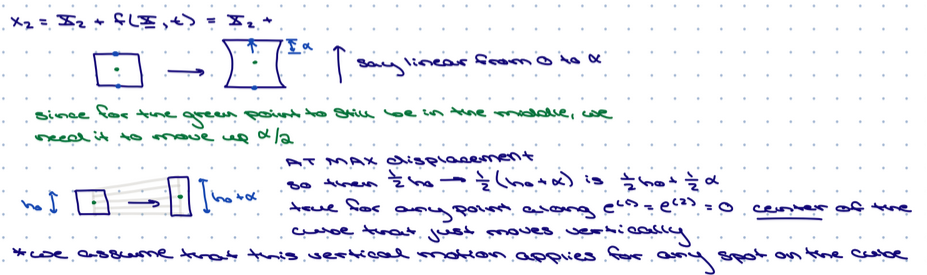
\includegraphics[scale=0.9]{Dawson-figures/1.png}

(An aside if that did not make sense in words: Expressed mathematically, if we consider the initial height of the HGC to be $h_0$, a point halfway up the initial cube is at $X_2 = \frac{1}{2}h_0$. The final height of the cube (at its maximum deformation) is then $h_0 + \alpha$, so for this point to remain halfway up the cube it is mapped to a final location of $x_2 = \frac{1}{2}(h_0 + \alpha) = \frac{1}{2}h_0 + \frac{1}{2}\alpha = X_2 + \frac{1}{2}\alpha$. So the point will move up by the same fraction of $\alpha$ that is its fraction of vertical height up the cube initially.)

This gives us the mapping function at maximum displacement of the cube, where we can note that the term $X_2 / h_0$ corresponds to the fraction "up that cube" that our initial material position is and that our initial height of the cube is $h_0 = 2$:
\begin{equation}
    x_2 = X_2 + \alpha \frac{X_2}{h_0} = X_2 + \alpha \frac{X_2}{2}
\end{equation}
Then putting in the sinusoidal dependence we get:
\begin{equation}
    x_2 = X_2 + \frac{\alpha X_2}{2} \sin{\omega t} = \chi_2(\bm{X},t)
\end{equation}

\emph{In the $\bm{e}^{(1)}$ and $\bm{e}^{(3)}$ directions}, we first note that the mapping functions should be the same. We also note that the displacement will be inwards, so a positive $X_1$ will have a negative change in position along $\bm{e}^{(1)}$ as it goes to $x_1$, and a negative $X_1$ will have a positive change in position along $\bm{e}^{(1)}$ as it goes to $x_1$. Once again, the mapping function will have the general form below, where $f(\bm{X},t)$ represents the change in position along $\bm{e}^{(1)}$:
\begin{equation}
    x_1 = X_1 + f(\bm{X},t)
\end{equation}

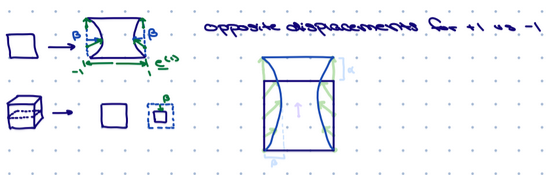
\includegraphics{Dawson-figures/2.png}

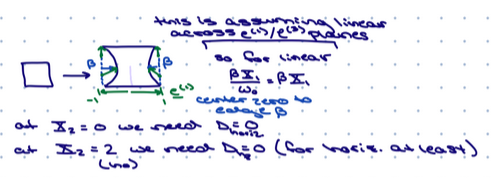
\includegraphics{Dawson-figures/3.png}

Along the center line ($X_1 = X_3 = 0$), $x_1 = X_1$ (ie. there is no lateral deformation). At the edge of the cube ($X_1 = X_3 = 1$) and halfway up the cube ($X_2 = 1$) there will be a maximum lateral deformation of $\beta$ ($x_1 = X_1 - \beta = 1-\beta$). We assume that all points in between are linearly related to these endpoints. That is, at $X_2 = 1$ we have a change in lateral position $-\beta X_1$. This gives us an equation for the maximum deformation thus far as:
\begin{equation}
    x_1 = X_1 - \beta X_1 X_2(t)
\end{equation}

The lateral displacement is also based on the vertical starting position, since at $X_2 = 0$ and $X_2 = 2$ we need $x_1 = X_1$ (no change in lateral position) with a maximum displacement in between these values. So, we also add in a parabolic function $X_2(t) = (X_2 - 2)(-x)$ to account for this dependence on vertical position. This gives us an expression for the maximum deformation:
\begin{equation}
    x_1 = X_1 + \beta X_1(X_2 - 2)(x)
\end{equation}
Where we can then add in the time-dependent sinusoidal dependence to get:
\begin{equation}
    x_1 = X_1 + \beta X_1(X_2 - 2)(x)\sin{\omega t} = \chi_1(\bm{X},t)
\end{equation}
Therefore, our overall mapping function $\bm{\chi}(\bm{X},t) = \bm{x}(t)$ is:
\begin{equation}
    \begin{split}
        x_1 = X_1 + \beta X_1(X_2 - 2)(x)\sin{\omega t} = \chi_1(\bm{X},t) \\
        x_2 = X_2 + \frac{\alpha}{2}X_2 \sin{\omega t} = \chi_2(\bm{X},t) \\
        x_3 = X_3 + \beta X_3(X_2 - 2)(x)\sin{\omega t} = \chi_3(\bm{X},t)
    \end{split}
\end{equation}

Then using this mapping function, we can calculate $\bn{F} = \gradX \space \bm{\chi}(\bm{X})$ by taking the corresponding partial derivatives of these components to get:

\begin{equation}
\bn{F} = 
\begin{bmatrix}
    1 + \beta X_2(X_2-2)\sin{\omega t} & \beta X_1 (2X_2-2)\sin{\omega t} & 0 \\
    0 & 1 + \frac{\alpha}{2}\sin{\omega t} & 0\\
    0 & \beta X_3 (2X_2-2)\sin{\omega t} & 1 + \beta X_2(X_2-2)\sin{\omega t}
\end{bmatrix}
\end{equation}
\hspace*{\fill} $\bigstar$

\medskip
(b) Determine the stretch magnitude of a small fiber positioned at a height $X_2 = 1$ and oriented at an angle $\theta$ from the $\bm{e}_1$ axis (in either the $\bm{e}_1- \bm{e}_2$ or $\bm{e}_1- \bm{e}_3$ plane). \newline
We first note that the stretch magnitude is $ \lambda (\bm{\hat{n}}) = \sqrt{\bm{\hat{n}} \cdot \bn{C} \bm{\hat{n}}}$ with $\bn{C} = \bn{F}^T\bn{F}$. Using our $\bn{F}$ from part (a), we note that $\bn{F}$ at $X_2 = 1$ is:
\begin{equation}
\bn{F} = 
\begin{bmatrix}
    1 - \beta \sin{\omega t} & 0 & 0 \\
    0 & 1 + \frac{\alpha}{2}\sin{\omega t} & 0\\
    0 & 0 & 1 - \beta \sin{\omega t}
\end{bmatrix}
\end{equation}
Which is also equal to $\bn{F}^T$ since it is a symmetric (and diagonal!) tensor. We can then calculate $\bn{C}$ as:
\begin{equation}
\bn{C} = \bn{F}^T\bn{F} = 
\begin{bmatrix}
    (1 - \beta \sin{\omega t})^2 & 0 & 0 \\
    0 & (1 + \frac{\alpha}{2}\sin{\omega t})^2 & 0\\
    0 & 0 & (1 - \beta \sin{\omega t})^2
\end{bmatrix}
\end{equation}
Then for $\bm{\hat{n}}$ in the $\bm{e}_1- \bm{e}_3$ plane we can note from the following sketch and some trigonometry that the unit vector should be:

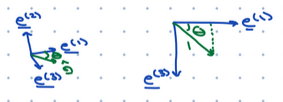
\includegraphics{Dawson-figures/BASIS.png}

\begin{equation}
    \bm{\hat{n}} = \cos{\theta}\bm{e}^{(1)} + 0\bm{e}^{(2)} + \sin{\theta}\bm{e}^{(3)}
\end{equation}
Then we can calculate $ \lambda (\bm{\hat{n}}) = \sqrt{\bm{\hat{n}} \cdot \bn{C} \bm{\hat{n}}}$ as follows:
\begin{equation}
    \bn{C}\bm{\hat{n}} = 
    \begin{bmatrix}
        \cos{\theta}(1 - \beta \sin{\omega t})^2 \\
        0 \\
         \sin{\theta}(1 - \beta \sin{\omega t})^2
    \end{bmatrix}
\end{equation}
\begin{equation}
    \bm{\hat{n}} \cdot \bn{C}\bm{\hat{n}} = 
        \cos^2{\theta}(1 - \beta \sin{\omega t})^2 + \sin^2{\theta}(1 - \beta \sin{\omega t})^2
\end{equation}
\begin{equation}
    \lambda (\bm{\hat{n}}) = \sqrt{\bm{\hat{n}} \cdot \bn{C} \bm{\hat{n}}} =  
        \sqrt{\cos^2{\theta}(1 - \beta \sin{\omega t})^2 + \sin^2{\theta}(1 - \beta \sin{\omega t})^2}
\end{equation}
Then we can simplify using the identity $\cos^2{\theta} + \sin^2{\theta} = 1$ to get:
\begin{equation}
    \lambda (\bm{\hat{n}}) = \sqrt{\bm{\hat{n}} \cdot \bn{C} \bm{\hat{n}}} =  
        \sqrt{ (\cos^2{\theta} + \sin^2{\theta})(1 - \beta \sin{\omega t})^2} = \sqrt{ (1 - \beta \sin{\omega t})^2} = (=1 - \beta \sin{\omega t}
\end{equation}
This is our $\lambda$ in the $\bm{e}_1- \bm{e}_3$ plane.
\hspace*{\fill} $\bigstar$

\medskip
(c) Determine the Lagrange-Green strain tensor $\bn{E}$ and the material logarithmic strain tensor $\bn{E}_H = \ln (\bn{U})$ for the geometric center $\bm{X}_c$ of the HGC. 
What are the maximum and minimum values of the strain eigenvalues $E_i(t)$ and $E_i^H(t)$? 
Would you expect one set to be more symmetric about zero as $\alpha$ gets large, and why? \newline
Note that the definition of the  Lagrange-Green strain tensor is $\bn{E} = \frac{1}{2}(\bn{C} - \bn{I})$. Using our $\bn{C}$ from part (b) we can calculate:
\begin{equation}
\bn{E} = (1/2) (
\begin{bmatrix}
    (1 - \beta \sin{\omega t})^2 & 0 & 0 \\
    0 & (1 + \frac{\alpha}{2}\sin{\omega t})^2 & 0\\
    0 & 0 & (1 - \beta \sin{\omega t})^2
\end{bmatrix} -
\begin{bmatrix}
    1 & 0 & 0 \\
    0 & 1 & 0\\
    0 & 0 & 1
\end{bmatrix} )
% \begin{bmatrix}
%     (1 - \beta \sin{\omega t})^2 -1 & 0 & 0 \\
%     0 & (1 + \frac{\alpha}{2}\sin{\omega t})^2 -1& 0\\
%     0 & 0 & (1 - \beta \sin{\omega t})^2 -1
% \end{bmatrix} )
\end{equation}

Performing this subtraction:
\begin{equation}
\bn{E} = (1/2)
\begin{bmatrix}
    (1 - \beta \sin{\omega t})^2 -1 & 0 & 0 \\
    0 & (1 + \frac{\alpha}{2}\sin{\omega t})^2 -1& 0\\
    0 & 0 & (1 - \beta \sin{\omega t})^2 -1
\end{bmatrix}
\end{equation}

Using that $a^2 - b^2 = (a+b)(a-b)$:
\begin{equation}
\bn{E} = (1/2)
\begin{bmatrix}
    (2 - \beta \sin{\omega t})(-\beta \sin{\omega t}) & 0 & 0 \\
    0 & (2 + \frac{\alpha}{2}\sin{\omega t})(\frac{\alpha}{2}\sin{\omega t})& 0\\
    0 & 0 & (2 - \beta \sin{\omega t})(-\beta \sin{\omega t})
\end{bmatrix}
\end{equation}
And applying the scalar multiplication by $1/2$ and simplifying:
\begin{equation}
\bn{E} =
\begin{bmatrix}
    (\beta \sin{\omega t}-2)(\frac{\beta}{2} \sin{\omega t}) & 0 & 0 \\
    0 & (2 + \frac{\alpha}{2}\sin{\omega t})(\frac{\alpha}{4}\sin{\omega t})& 0\\
    0 & 0 & (\beta \sin{\omega t}-2)(\frac{\beta}{2} \sin{\omega t})
\end{bmatrix}
\end{equation}
\hspace*{\fill} $\bigstar$

Note that the definition of the  material logarithmic strain tensor is $\bn{E}_H = \ln (\bn{U})$ with $\bn{U}$ the right stretch tensor. Since $\bn{C} = \bn{F}^T\bn{F} = \bn{U}^2$ and $\bn{F}$ is symmetric for the geometric center $\bn{X}_C$ (since there $X_2 = 1$, so it is the same simplified $\bn{F}$ as in part (b)) we can note that $\bn{C} = \bn{F}^2 = \bn{U}^2$ so $\bn{F} = \bn{U}$.
\begin{equation}
\bn{F} = \bn{U} =
\begin{bmatrix}
    1 - \beta \sin{\omega t} & 0 & 0 \\
    0 & 1 + \frac{\alpha}{2}\sin{\omega t} & 0\\
    0 & 0 & 1 - \beta \sin{\omega t}
\end{bmatrix}
\end{equation}
Then $\bn{E}_H = \ln (\bn{F})$ with $\bn{F}$ also a diagonal matrix, so we can just take the natural log of the diagonal components.
\begin{equation}
\bn{E}_H =\ln
\begin{bmatrix}
    1 - \beta \sin{\omega t} & 0 & 0 \\
    0 & 1 + \frac{\alpha}{2}\sin{\omega t} & 0\\
    0 & 0 & 1 - \beta \sin{\omega t}
\end{bmatrix} = 
\begin{bmatrix}
    \ln(1 - \beta \sin{\omega t}) & 0 & 0 \\
    0 & \ln(1 + \frac{\alpha}{2}\sin{\omega t}) & 0\\
    0 & 0 & \ln(1 - \beta \sin{\omega t})
\end{bmatrix}
\end{equation}
\hspace*{\fill} $\bigstar$

Then, for the minimum and maximum eigenvalues, we first note that these are both diagonal matrices and that the eigenvalues of a diagonal matrix will be the entries along the diagonal.

For $\bn{E}$, the eigenvalues are $\{(\beta \sin{\omega t}-2)(\frac{\beta}{2} \sin{\omega t}), (2 + \frac{\alpha}{2}\sin{\omega t})(\frac{\alpha}{4}\sin{\omega t}) \}$. To find the minimum and maximum eigenvalues, we check the extreme values of $\sin{\omega t}$, $\beta$, and $\alpha$. For the purposes of making this problem physically reasonable, assume that we can have $\beta$ values from $[0,1]$ and $\alpha$ values from $[0,2]$ (a maximum reasonable $\alpha$ of $2\beta$). $\sin{\omega t}$ will be on the domain $[-1,1]$.

For $\sin{\omega t} = 0$ we have eigenvalues $\{0, 0\}$.

For $\sin{\omega t} = 1$ we have eigenvalues $\{(\beta-2)(\beta/2), (2+\alpha/2)(\alpha/4)\}$. For $\beta = 0$ we get a first eigenvalue of $0$. For $\beta = 1$ we get a first eigenvalue of $-1/2$. For $\alpha = 0$ we get a second eigenvalue of $0$. For $\alpha = 2$ we get a second eigenvalue of $3/2$.

For $\sin{\omega t} = -1$ we have eigenvalues $\{(-\beta-2)(-\beta/2), (2-\alpha/2)(-\alpha/4)\}$ For $\beta = 0$ we get a first eigenvalue of $0$. For $\beta = 1$ we get a first eigenvalue of $3/2$. For $\alpha = 0$ we get a second eigenvalue of $0$. For $\alpha = 2$ we get a second eigenvalue of $-1/2$.

So our maximum eigenvalue for $\bn{E}$ is $3/2$ and our minimum is $-1/2$. As $\alpha$ gets large (say $\alpha \to \infty$) our maximum eigenvalue also goes to $\infty$ but our minimum remains as $-1/2$.
\hspace*{\fill} $\bigstar$

For $\bn{E}_H$, the eigenvalues are $\{\ln(1-\beta\sin{\omega t}), \ln(1+\frac{\alpha}{2}\sin{\omega t}) \}$. Repeating a similar process we get the following.

For $\beta = 0$ we have a first eigenvalue of $0$.

For $\beta = 1$ we have a first eigenvalue $\ln(1-\sin{\omega t})$. For $\sin{\omega t} = 0$ we have a first eigenvalue $\ln(1)=0$. For $\sin{\omega t} = 1$ we have a first eigenvalue $\ln(2)$. For $\sin{\omega t} = -1$ we have a first eigenvalue $\ln(0)=-\infty$.

For $\alpha = 0$ we have a first eigenvalue of $0$.

For $\alpha = 2$ we have a first eigenvalue $\ln(1+\sin{\omega t})$. For $\sin{\omega t} = 0$ we have a first eigenvalue $\ln(1)=0$. For $\sin{\omega t} = 1$ we have a first eigenvalue $\ln(2)$. For $\sin{\omega t} = -1$ we have a first eigenvalue $\ln(0)=-\infty$.

So our maximum eigenvalue for $\bn{E}_H$ is $\ln(2)$ and our minimum is $-\infty$. As $\alpha$ gets large (say $\alpha \to \infty$) our maximum eigenvalue goes to $\infty$ and our minimum remains $-\infty$. This also means that $\bn{E}_H$ has a more symmetric set of eigenvalues about zero as $\alpha$ gets large.
\hspace*{\fill} $\bigstar$

\medskip
(d) Determine both the material point acceleration $\bm{A}(\bm{X}_1)$ at a point $\frac{1}{2} \bm{e}_1 + 2\bm{e}_2 + \frac{1}{2} \bm{e}_3$.  
The material point acceleration is defined as:
\begin{equation}
    \bm{A}(\bm{X},t) = \frac{\partial^2 \bm{\chi}}{\partial t^2}
\end{equation}
With components $A_i = \frac{\partial^2 \bm{\chi}_i}{\partial t^2}$.
Taking our second derivatives of each component for the mapping function we get:
\begin{equation}
\begin{split}
    A_1 = \frac{\partial^2}{\partial t^2} (X_1 + \beta X_1(X_2 - 2)(x)\sin{\omega t}) = -\beta \omega^2 X_1X_2(X_2-2)(\sin{\omega t}) \\
    A_2 = \frac{\partial^2}{\partial t^2} (X_2 + \frac{\alpha}{2}X_2 \sin{\omega t}) = -(\alpha /2)X_2\omega^2(\sin{\omega t}) \\
    A_3 = \frac{\partial^2}{\partial t^2} (X_3 + \beta X_3(X_2 - 2)(x)\sin{\omega t}) = -\beta \omega^2 X_3X_2(X_2-2)(\sin{\omega t})
\end{split}
\end{equation}
Evaluating this at the material point $\bm{X} = \frac{1}{2} \bm{e}_1 + 2\bm{e}_2 + \frac{1}{2} \bm{e}_3$, so components $X_1 = 1/2$, $X_2 = 2$, and $X_3 = 1/2$, we get:
\begin{equation}
\begin{split}
    A_1 = 0 \\
    A_2 = -\alpha \omega^2\sin{\omega t} \\
    A_3 = 0
\end{split}
\end{equation}
Giving us a material point acceleration vector of:
\begin{equation}
    \bm{A} = 0 \bm{e}_1 -\alpha \omega^2\sin{\omega t}\bm{e}_2 + 0\bm{e}_3
\end{equation}
\hspace*{\fill} $\bigstar$

% \end{document}

\end{document}

% Section 1 Notes
% by which the VE properties of MTs are established microtubules vary in exhibiting these properties

%These results indicate that individual microtubules might also exhibit viscoelastic behaviors.
%as well as a decreased persistence length
%individual \C{deacetylated} microtubules showed an increase in deformation 

% importnat for understanding networks and deformations over time? where would a MT act more independently rather than in a bundle though, or why would the single molecule mechanical properties actually matter?
% However, recent papers have demonstrated that individual microtubules might exhibit viscoelastic behaviors

% Microtuuuuuuuubles.
% Looking at them from a viscoelastic perspective, particularly in terms of relaxation.
% Single microtubules, but could also do networks or bundles that have already been looked at as viscoelastic?